\documentclass[utf8,bachelor]{gradu3}
%DIF LATEXDIFF DIFFERENCE FILE


% If you are writing a Bachelor's Thesis, use the following instead:
%\documentclass[utf8,bachelor,english]{gradu3}

\usepackage{graphicx} % for including pictures

\usepackage{amsmath} % useful for math (optional)

\usepackage{booktabs} % good for beautiful tables

% NOTE: This must be the last \usepackage in the whole document!
\usepackage[bookmarksopen,bookmarksnumbered,linktocpage]{hyperref}

\addbibresource{references.bib} % The file name of your bibliography database
%DIF PREAMBLE EXTENSION ADDED BY LATEXDIFF
%DIF UNDERLINE PREAMBLE %DIF PREAMBLE
\RequirePackage[normalem]{ulem} %DIF PREAMBLE
\RequirePackage{color}\definecolor{RED}{rgb}{1,0,0}\definecolor{BLUE}{rgb}{0,0,1} %DIF PREAMBLE
\providecommand{\DIFaddtex}[1]{{\protect\color{blue}\uwave{#1}}} %DIF PREAMBLE
\providecommand{\DIFdeltex}[1]{{\protect\color{red}\sout{#1}}}                      %DIF PREAMBLE
%DIF SAFE PREAMBLE %DIF PREAMBLE
\providecommand{\DIFaddbegin}{} %DIF PREAMBLE
\providecommand{\DIFaddend}{} %DIF PREAMBLE
\providecommand{\DIFdelbegin}{} %DIF PREAMBLE
\providecommand{\DIFdelend}{} %DIF PREAMBLE
%DIF FLOATSAFE PREAMBLE %DIF PREAMBLE
\providecommand{\DIFaddFL}[1]{\DIFadd{#1}} %DIF PREAMBLE
\providecommand{\DIFdelFL}[1]{\DIFdel{#1}} %DIF PREAMBLE
\providecommand{\DIFaddbeginFL}{} %DIF PREAMBLE
\providecommand{\DIFaddendFL}{} %DIF PREAMBLE
\providecommand{\DIFdelbeginFL}{} %DIF PREAMBLE
\providecommand{\DIFdelendFL}{} %DIF PREAMBLE
%DIF HYPERREF PREAMBLE %DIF PREAMBLE
\providecommand{\DIFadd}[1]{\texorpdfstring{\DIFaddtex{#1}}{#1}} %DIF PREAMBLE
\providecommand{\DIFdel}[1]{\texorpdfstring{\DIFdeltex{#1}}{}} %DIF PREAMBLE
\newcommand{\DIFscaledelfig}{0.5}
%DIF HIGHLIGHTGRAPHICS PREAMBLE %DIF PREAMBLE
\RequirePackage{settobox} %DIF PREAMBLE
\RequirePackage{letltxmacro} %DIF PREAMBLE
\newsavebox{\DIFdelgraphicsbox} %DIF PREAMBLE
\newlength{\DIFdelgraphicswidth} %DIF PREAMBLE
\newlength{\DIFdelgraphicsheight} %DIF PREAMBLE
% store original definition of \includegraphics %DIF PREAMBLE
\LetLtxMacro{\DIFOincludegraphics}{\includegraphics} %DIF PREAMBLE
\newcommand{\DIFaddincludegraphics}[2][]{{\color{blue}\fbox{\DIFOincludegraphics[#1]{#2}}}} %DIF PREAMBLE
\newcommand{\DIFdelincludegraphics}[2][]{% %DIF PREAMBLE
\sbox{\DIFdelgraphicsbox}{\DIFOincludegraphics[#1]{#2}}% %DIF PREAMBLE
\settoboxwidth{\DIFdelgraphicswidth}{\DIFdelgraphicsbox} %DIF PREAMBLE
\settoboxtotalheight{\DIFdelgraphicsheight}{\DIFdelgraphicsbox} %DIF PREAMBLE
\scalebox{\DIFscaledelfig}{% %DIF PREAMBLE
\parbox[b]{\DIFdelgraphicswidth}{\usebox{\DIFdelgraphicsbox}\\[-\baselineskip] \rule{\DIFdelgraphicswidth}{0em}}\llap{\resizebox{\DIFdelgraphicswidth}{\DIFdelgraphicsheight}{% %DIF PREAMBLE
\setlength{\unitlength}{\DIFdelgraphicswidth}% %DIF PREAMBLE
\begin{picture}(1,1)% %DIF PREAMBLE
\thicklines\linethickness{2pt} %DIF PREAMBLE
{\color[rgb]{1,0,0}\put(0,0){\framebox(1,1){}}}% %DIF PREAMBLE
{\color[rgb]{1,0,0}\put(0,0){\line( 1,1){1}}}% %DIF PREAMBLE
{\color[rgb]{1,0,0}\put(0,1){\line(1,-1){1}}}% %DIF PREAMBLE
\end{picture}% %DIF PREAMBLE
}\hspace*{3pt}}} %DIF PREAMBLE
} %DIF PREAMBLE
\LetLtxMacro{\DIFOaddbegin}{\DIFaddbegin} %DIF PREAMBLE
\LetLtxMacro{\DIFOaddend}{\DIFaddend} %DIF PREAMBLE
\LetLtxMacro{\DIFOdelbegin}{\DIFdelbegin} %DIF PREAMBLE
\LetLtxMacro{\DIFOdelend}{\DIFdelend} %DIF PREAMBLE
\DeclareRobustCommand{\DIFaddbegin}{\DIFOaddbegin \let\includegraphics\DIFaddincludegraphics} %DIF PREAMBLE
\DeclareRobustCommand{\DIFaddend}{\DIFOaddend \let\includegraphics\DIFOincludegraphics} %DIF PREAMBLE
\DeclareRobustCommand{\DIFdelbegin}{\DIFOdelbegin \let\includegraphics\DIFdelincludegraphics} %DIF PREAMBLE
\DeclareRobustCommand{\DIFdelend}{\DIFOaddend \let\includegraphics\DIFOincludegraphics} %DIF PREAMBLE
\LetLtxMacro{\DIFOaddbeginFL}{\DIFaddbeginFL} %DIF PREAMBLE
\LetLtxMacro{\DIFOaddendFL}{\DIFaddendFL} %DIF PREAMBLE
\LetLtxMacro{\DIFOdelbeginFL}{\DIFdelbeginFL} %DIF PREAMBLE
\LetLtxMacro{\DIFOdelendFL}{\DIFdelendFL} %DIF PREAMBLE
\DeclareRobustCommand{\DIFaddbeginFL}{\DIFOaddbeginFL \let\includegraphics\DIFaddincludegraphics} %DIF PREAMBLE
\DeclareRobustCommand{\DIFaddendFL}{\DIFOaddendFL \let\includegraphics\DIFOincludegraphics} %DIF PREAMBLE
\DeclareRobustCommand{\DIFdelbeginFL}{\DIFOdelbeginFL \let\includegraphics\DIFdelincludegraphics} %DIF PREAMBLE
\DeclareRobustCommand{\DIFdelendFL}{\DIFOaddendFL \let\includegraphics\DIFOincludegraphics} %DIF PREAMBLE
%DIF END PREAMBLE EXTENSION ADDED BY LATEXDIFF

\begin{document}

\title{Lohkoketju - konsensus ja haasteet}
\translatedtitle{Blockchain - consensus and challenges}
\studyline{Tietotekniikka}
\DIFdelbegin %DIFDELCMD < \avainsanat{%
%DIFDELCMD <   lohkoketju,
%DIFDELCMD <   älysopimus,
%DIFDELCMD <   konsensus-algoritmi,
%DIFDELCMD <   lohkoketjujen ongelmat
%DIFDELCMD <   }
%DIFDELCMD < \keywords{
%DIFDELCMD <     blockchain,
%DIFDELCMD <     smart contract,
%DIFDELCMD <     consensus algorithm,
%DIFDELCMD <     blockchains problems
%DIFDELCMD < }
%DIFDELCMD < %%%
\DIFdelend \DIFaddbegin \avainsanat{%
  lohkoketju,
  konsensus-algoritmi,
  lohkoketjujen ongelmat
  }
\keywords{
    blockchain,
    consensus algorithm,
    blockchains problems
}
\DIFaddend \tiivistelma{%

}
\abstract{%

}

\author{Niko Sihvo}
\contactinformation{\texttt{niko.m.sihvo@student.jyu.fi}}
% use a separate \author command for each author, if there is more than one
\DIFdelbegin %DIFDELCMD < \supervisor{Unsupervised work}
%DIFDELCMD < %%%
\DIFdelend \DIFaddbegin \supervisor{Tuomo Rossi}
\DIFaddend % use a separate \supervisor command for each supervisor, if there
% is more than one

 % you don't need this line in a thesis
% \type{Template and manual for a thesis document class}

\maketitle


\begin{thetermlist}
\item[lohko] Lohkoketjun perustan muodostavien transaktioiden kokoelma.
\item[lohkoaika] Keskimääräinen aika mitä uuden lohkon luomiseen kuluu.
\item[node] Yksittäinen käyttäjä lohkoketjuverkossa
\item[louhija] Node, joka luo uusia lohkoja
\item[louhinta] Prosessi, jossa uusi lohko lisätään lohkoketjuun 
\item[DLT] Distributed Ledger Technology
\item[dApp] Decentralized Application
\item[NFT] Non-Fungible Token
\item[GDPR] The European General Data Protection Regulation
\end{thetermlist}

\mainmatter

\chapter{Johdanto}

Lohkoketjuteknologiat ovat saaneet viime vuosina huomattavan suosion, varsinkin kryptovaluuttojen muodossa. Lohkoketjuteknologiaa voidaan käyttää muihinkin kuin finanssialan toimiin, kuten logistiikkaan. 
Ideaalisessa tilanteessa lohkoketjut puoltaisi hajautettua, läpinäkyvää sekä demokraattisempaa internettiä.

Luvussa \ref{Lohkoketju} tarkastellaan lohkoketjun toimintaperiaatteita ja miten lohkoketjut on saanut lähtönsä.
\ref{Konsensus} luku tarkastelee pintapuolisesti potentiaalisia sekä suosituimpia konsensus-algoritmeja.
Lopuksi luvussa \ref{Haasteet} käydään läpi lohkoketjujen kohtaamia haasteita.



\chapter{Lohkoketju}\label{Lohkoketju}
\section{Historia}

Lohkoketjuteknologian perusajatus on lähtöisin 80- ja 90-luvun vaihteesta, jolloin Leslie Lamport kehitti Paxos protokollan. 
Tutkielmassa kuvaillaan konsensusmalli, missä verkkoon liitetyt tietokoneet voivat tulla yhteisymmärrykseen epäluotettavassa ympäristössä \DIFaddbegin \parencite{lamport2019part}\DIFaddend . 
Vuonna 1991 otettiin käyttöön allekirjoitettu tietoketju elektronisena kirjanpitona dokumenttien digitaalisessa allekirjoittamisessa. Tietoketjusta nähtiin helposti kuka on muokannut dokumenttia digitaalisena jälkenä.

Nämä kaksi konseptia sovellettiin yhteen luoden ensimmäisen lohkoketjusovelluksen Bitcoinin. Bitcoin esiteltiin Satoshi Nakamoton artikkelissa \parencite{nakamoto2008bitcoin}.
Nakamoton artikkeli on monien modernien kryptovaluuttojen perusta.
Bitcoin on myös ensimmäisiä menestyneitä lohkoketjusovelluksia.


\section{Perusperiaatteet}

\begin{figure}[h]\centering
  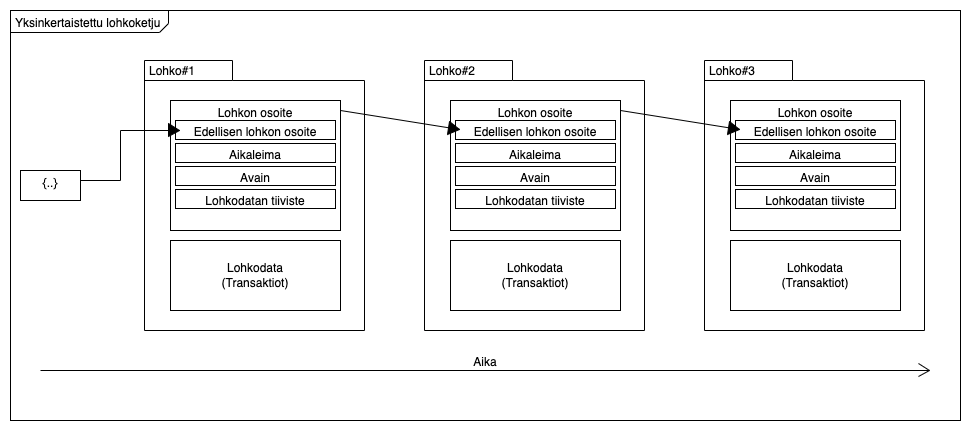
\includegraphics[height=7cm,keepaspectratio]{lohkoketjuDiag}
  \caption[Yksinkertainen lohkoketju]{Yksinkertainen lohkoketju}
  \label{fig:Lohkoketju}
\end{figure}

\DIFdelbegin \DIFdel{\mbox{%DIFAUXCMD
\cite{yaga2019blockchain} }\hspace{0pt}%DIFAUXCMD
määritelee tiivistetysti lohkoketjun seuraavasti. Lohkoketjut ovat hajautettja }\DIFdelend \DIFaddbegin \DIFadd{Lohkoketjut ovat hajautettuja }\DIFaddend digitaalisia tilikirjoja, \DIFdelbegin \DIFdel{mitkä }\DIFdelend \DIFaddbegin \DIFadd{jotka }\DIFaddend sisältävät \DIFaddbegin \DIFadd{lohkoihin ryhmiteltyjä }\DIFaddend kryptograafisesti allekirjoitettuja transaktioita \DIFdelbegin \DIFdel{, jotka ovat ryhmitetty lohkoihin}\DIFdelend \DIFaddbegin \parencite{yaga2019blockchain}\DIFaddend .
Jokainen lohko on \DIFdelbegin \DIFdel{kryptograafisesti linkitetty edelliseen}\DIFdelend \DIFaddbegin \DIFadd{linkitetty kryptograafisesti edelliseen validoinnin ja konsensuksen jälkeen lohkoon}\DIFaddend , mikä tekee \DIFdelbegin \DIFdel{lohkosta peukaloinnilta vapaan, validoinnin ja konsensus-algoritmin jälkeen}\DIFdelend \DIFaddbegin \DIFadd{lohkoista peukaloinnilta vapaan}\DIFaddend .
Kun uusia lohkoja liitetään ketjuun, vanhoja lohkoja on entistä vaikeampi muokata. 
Uudet lohkot toisinnetaan lohkoketjuverkon kopioiden kanssa ja mahdolliset konfliktit ratkaistaan automaattisesti käyttäen luotuja sääntöjä.

%DIF >  Tee kaavio prosessista tähän
\DIFaddbegin 

\DIFaddend Lohkoketjun ensisijainen hyöty on mahdollistaa suorat transaktiot käyttäjien välillä ilman kolmansia osapuolia \parencite{yaga2019blockchain}.
Lohkoketjuissa yleisesti palkitkaan \DIFaddbegin \DIFadd{louhijoita eli }\DIFaddend käyttäjiä, \DIFdelbegin \DIFdel{jotka }\DIFdelend \DIFaddbegin \DIFadd{ketkä }\DIFaddend julkaisevat uusia lohkoja ketjuun ja \DIFdelbegin \DIFdel{ylläpitää }\DIFdelend \DIFaddbegin \DIFadd{ylläpitävät }\DIFaddend tilikirjan kopiota.
\DIFdelbegin \DIFdel{Tälläisiä käyttäjiä kutsutaan louhijoiksi.
}\DIFdelend Louhijoiden automatisoitu maksu mahdollistaa systeemin hajautetun hallinnon ilman kolmansia osapuolia.
Tämä lohkoketjujärjestelmän käyttäjien itsevalvottu mekanismi, konsensus-algoritmi, vakuuttaa, että vain validit transaktiot ja lohkot lisätään lohkoketjuun.
Lohkoketjujen \DIFdelbegin \DIFdel{käyttö }\DIFdelend \DIFaddbegin \DIFadd{käyttäminen }\DIFaddend mahdollistaa tilan, missä yksittäinen käyttäjä ei ohjaa \DIFdelbegin \DIFdel{elektronista rahaa }\DIFdelend \DIFaddbegin \DIFadd{transaktiota }\DIFaddend eikä järjestelmässä ole yksittäistä epäonnistumispistettä.

\DIFdelbegin \DIFdel{Bitcoinissa }\DIFdelend \DIFaddbegin \DIFadd{Yleisesti }\DIFaddend käyttäjät ovat pseudoanonyymeja, mutta heidän käyttäjätunnisteet eivät ole\DIFdelbegin \DIFdel{, lisäksi }\DIFdelend \DIFaddbegin \DIFadd{. 
Lisäksi }\DIFaddend kaikki transaktiot ovat julkisia. 
Koska lohkoketjutsovellukset ovat yleensä salattuja, on olennaista olla \DIFdelbegin \DIFdel{mekanismit }\DIFdelend \DIFaddbegin \DIFadd{keinot }\DIFaddend luottamuksen luotiin ympäristössä, jossa käyttäjiä ei voi tunnistaa suoraan. 
\DIFaddbegin \DIFadd{Käyttäjä ei voi olla täysin anonyymi kuluttujansuojalakien takia.   
}\DIFaddend \parencite{yaga2019blockchain}
\DIFdelbegin \DIFdel{Ennen lohkoketjuja, }\DIFdelend \DIFaddbegin \DIFadd{Perinteisesti }\DIFaddend käyttäjien välinen luottamus \DIFdelbegin \DIFdel{toteutettiin }\DIFdelend \DIFaddbegin \DIFadd{toteutetaan }\DIFaddend molempien osapuolien luottaman välikäden kautta, kuten pankki \DIFaddbegin \DIFadd{kautta}\DIFaddend .
Ilman luotettavia välikäsiä, lohkoketjussa luottamus luodaan seuraavan neljän avainominaisuuden kautta \parencite{zarrin2021blockchain}.

Hajautus, missä jokainen lohkoketjuverkossa tehdyt transaktiot tehdään vain kahden noden välillä kerrallaan ilman kolmansia osapuolia. Hajautuminen mahdollistaa lohkoketjujen käytön ilman riippumattomia keskitettyjä viranomaisia. Tällöin jokaisella nodella on periaatteessa yhtäläiset äänestysoikeudet lohkoketjuverkossa.

Muuttumattomuus \DIFdelbegin \DIFdel{, mikä }\DIFdelend viittaa siihen että transaktio täytyy validoida luotetuilla louhijoilla. Muuttumattomuus vakuuttaa, että nodeihin tallennetut tilikirjat pysyy absoluuttisina eikä niitä pysty poistamaan.

Anonymiteetti, \DIFdelbegin \DIFdel{joka viittaa jokaisen louhija generoitua osoitetta }\DIFdelend \DIFaddbegin \DIFadd{viittaa jokaisen louhijan generoituun osoitteeseen }\DIFaddend uniikkina indentiteettinä.
Vaikka kaikki lohkoketjut ei ole anonyymeja kokonaan ja jotkut harjoittaa pseudo-anonymiteettiä, kuten Bitcoin ja Ethereum, missä osoitteet generoidaan jokaisessa lohkoketjun transaktiossa. 

Tarkastettavuus, missä jokaisella transaktiolla on oma viite lohkoketjussa, mikä \DIFaddbegin \DIFadd{on }\DIFaddend myös \DIFdelbegin \DIFdel{tallennetaan }\DIFdelend \DIFaddbegin \DIFadd{tallennettu }\DIFaddend lohkoketjun nodeihin. Näitä viitteitä käytetään jokaisen varmennetun transaktion aktivointiin ja jäljittämiseen lohkoketjussa. Näin jokaisesta transaktiosta jää merkki lohkoketjuverkkoon.



\section{Komponentit}
Lohkoketjut sisältävät kolme pakollista pääkomponenttia, jotka ovat DLT, muuttumaton tilikirja ja konsensus-algoritmit \parencite{zarrin2021blockchain}.

DLT tarjoaa hajautetun tietokannan, joka muodostaa internetyhteyden käyttäjien välille. Tietokoneita joita käytetään yhteyksien luontiin kutsutaan nodeiksi.
Nodet sisältävät tilikirjan, joka on järjestetty lista aikaleimatuista transaktioista.
Tilikirjaa voi laajentaa vain tietokannalla, mikä mahdollistaaa turvallisen keinon jäljittää transaktoita ilman keskitettyä tarkastusta.

Muuttumattomalla tilikirjalla viitataan nodejen kykyyn olla muuttumatton.
Jokainen tilikirjaa on tallennettu jokaiseen nodeen ja tilikirjalla on viite itseensä lohkoketjussa muuttumattomana historiana.
Muuttumattomassa tilikirjassa käytetään salausfunktiota tilikirjojen eheyden ylläpitoon nodeissa.
Muuttumattomuus takaa etteivät muut välikädet pysty muokkaamaan transaktioiden sisältöä.

Konsensus-algoritmeja käytetään saavuttamaan yhteisymmärrys nodejen välillä, kun yritetään lisätä uutta lohkoa lohkoketjun loppuun.
Konsensus-algoritmi moderoi lohkoketjua sanelemalla nodeja kuinka päästä yhteisymmärrykseen ja päivittää lohkoketjuverkkoa. Lisää konsensus-algoretmeista luvusssa 5.

\DIFaddbegin \section{\DIFadd{Tiivistefunktio}}
\DIFadd{Lohkoketjut käyttävät tiivistefunktioita lohkojen ketjuttamiseen ja tiedon salaukseen. Jokaisella lohkolla on tiiviste osoitteena, mikä on generoitu lohkon sisällön mukaan. 
Tiiviste on yksisuuntainen kryptografinen funktio.
Tiivistefunktio ottaa yleisesti rajattoman määrän syötettä ja tulostaa lopulta tietyn pituisen merkkijonon. Jokainen tuloste on uniikki tietylle syötteelle.
Jos syötettä muutetaan merkilläkin, niin tuloste muuttuu täysin.
Täten jos lohkon sisältöä muuttaa, osoite muuttuu myös, mikä tekee validoiduista lohkoista muuttumattomia.
}


\DIFaddend \section{Kategoriat}
Lohkoketjut voidaan kategorisoida kahteen joukkoon, luvattomiin ja luvallisiin.

Luvaton lohkoketjuverkko on kaikille avoin hajauttettu tilikija alusta. 
Jokainen käyttäjä pystyy liittämään uuden lohkon lohkoketjuun ilman ylempien tahojen lupaa. Yleisesti luvattomat lohkoketjut on avointa lähdekoodia.
Koska kaikilla luvattoman lohkoketjun käyttäjillä on lupa kirjoittaa lohkoketjuun on heillä myös oikeus lukea lohkoketjua\DIFdelbegin \DIFdel{myös}\DIFdelend .
Koska jokainen käyttäjä voi julkaista lohkoja luvattomassa lohkoketjussa, haitalliset käyttäjät voivat yrittää julkaista valheellista dataa lohkoketjuun.
\DIFdelbegin \DIFdel{Tosin konsensus-algoritmit vaikeuttavat }\DIFdelend \DIFaddbegin \DIFadd{Konsensus-algoritmi vaikeuttaa }\DIFaddend haitallisten käyttäjien yrityksiä korruptoida lohkoketjua huomattavasti.
Luvaton lohkoketjuverkko kannustaa yleensä ilkivallattomaan toimintaan palkitsemalla lohkojen julkaisijoille lohkoketjun omaa kryptovaluutta.

Luvallisissa vain \DIFdelbegin \DIFdel{tietyt }\DIFdelend \DIFaddbegin \DIFadd{valitut }\DIFaddend käyttäjät voivat liittää lohkoja lohkoketjuun \DIFdelbegin \DIFdel{jonkun }\DIFdelend hajautetun tai keskitetyn viranomaisen toimesta.
Koska vain \DIFdelbegin \DIFdel{luvansaaneet }\DIFdelend \DIFaddbegin \DIFadd{luvan saaneet }\DIFaddend käyttäjät ylläpitävät lohkoketjua, on mahdollista rajoittaa luku- ja kirjoitusoikeuksia.
Luvallisissa lohkoketjuverkkoissa on samat ominaisuudet kuin luvattomassa lohkoketjussa.
\DIFdelbegin \DIFdel{Luvallinen lohkoketju käyttää }\DIFdelend \DIFaddbegin \DIFadd{Luvalliset lohkoketjut käyttävöt siis }\DIFaddend myös \DIFdelbegin \DIFdel{konsensus algoritmeja lohkojen julkaisemiseen}\DIFdelend \DIFaddbegin \DIFadd{konsensus-algoritmeja lohkojen liittämiseen}\DIFaddend , mutta yleensä käytössä ei ole yhtä raskaita algoritmeja, koska luvallisen lohkoketjun käyttäjillä on luottamusta toisiinsa. Luottamus perustuu \DIFdelbegin \DIFdel{sihhen }\DIFdelend \DIFaddbegin \DIFadd{siihen }\DIFaddend että käyttäjät ovat \DIFdelbegin \DIFdel{luvan }\DIFdelend \DIFaddbegin \DIFadd{saaneet luvan lohkoketjuun }\DIFaddend ylemmältä taholta\DIFdelbegin \DIFdel{lohkoketjuun}\DIFdelend .

\section{Tyypit}

\DIFaddbegin \DIFadd{Lohkoketjun tyypin voi jakaa kolmeen joukkoon, julkinen, hybridi sekä yksityinen. Lohkoketjun tyyppi määritteleen ketkä osasllistuvat varmennukseen ja konsensusprosessiin. 
}

\DIFaddend %\subsection{Julkinen lohkoketju}
Julkisessa lohkoketjussa jokainen osallistuja osallistuu lohkoketjun varmennukseen ja konsensusprosessiin. Julkinen lohkoketju on yleisesti luvaton lohkoketju, missä nodet voivat liittyä lohkoketjuun ilman erillisiä lupia. Nodeilla on täydet oikeudet lukea lohkoketjua ja kirjoittaa julkiseen lohkoketjuun.

%\subsection{Hybridilohkoketju}
Hybridilohkoketjussa vain valitut nodet julkisen tai yksityisen lohkoketjun haarasta pystyvät käsittelemään lohkoketjun varmennuksen ja \DIFdelbegin \DIFdel{konsensus prosessin}\DIFdelend \DIFaddbegin \DIFadd{konsensusprosessin}\DIFaddend . Hybridilohkoketju luokitellaan luvalliseksi lohkoketjuksi, koska se hyödyntää samaa logiikkaa todentamisessa, jossa vain rajatulla määrällä nodeja on luku- ja kirjoitusoikeudet.

%\subsection{Yksityinen lohkoketju}
Yksityinen lohkoketju käyttää yksityisiä nodeja organisaatiossa tai ryhmästä, joka on rajattu julkisuudelta, lohkoketjun varmennukseen ja konsensusprosessiin. Noden oikeuksia pystytään rajaamaan siten että node ei pysty osallistumaan molempiin prosesseihin, vaikka node kuuluisikin samaan organisaatioon tai ryhmään.  Yksityinen lohkoketju on luvallinen lohkoketju, mikä toimii samalla periaatteella valittujen nodejen kanssa kuten hybridilohkoketju. Se miten yksityinen lohkoketju eroaa hybridilohkoketjusta on siten että \DIFdelbegin \DIFdel{hybridilohkoketjussa }\DIFdelend \DIFaddbegin \DIFadd{hybridimallissa }\DIFaddend nodet vahvistetaan useiden eri ryhmien toimesta, kun taas yksityisessä lohkoketjussa noden vahvistaa yksittäinen ryhmä, kuten organisaatio.

\begin{table}[ht]\centering
  \begin{tabular}{llll}
    \toprule
    Ominaisuudet & Julkinen & Hybridi & Yksityinen \\
    \midrule
    Konsensus & Kaikilla & Valituilla & Organisaatiolla \\
    Lukuoikeudet & Julkinen & Julkinen \& Yksityinen & Julkinen \& Yksityinen \\
    Muuttumattomuus & Lähes muuttumaton & Voidaan kajota & Voidaan kajota \\
    Tehokkuus & Matala & Korkea & Korkea \\
    Hajautuminen & Kyllä & Osittain & Ei \\
    Konsensus prosessi & Luvaton & Luvallinen & Luvallinen \\
    \bottomrule
  \end{tabular}
  \caption{Lohkoketjutyyppien vertailu - \cite{zarrin2021blockchain} - CC BY 4.0 - Muokattu}
  \label{tbl:cmdchange}
\end{table}

\section{Älysopimus}
Älysopimus on 1990 luvulla Nick Szabon esittelmä tietokoneprotokolla. Älysopimukset ovat ohjelmoituja sopimuslausekkeita, jotka toteutetaan, kun ennalta määritellyt ehdot täyttyvät.
Lohkoketjut mahdollistivat älysopimuksien käytön uudella tavalla, jossa sopimukset toteutetaan lohkoketjun päällä.
Jokainen älysopimuksessa suoritettu transaktio tallennetaan muuttumattomana lohkoketjuun, mikä tekee transaktioista jäljitettäviä ja peruuttamattomia. 
\DIFdelbegin \DIFdel{Älysopimuksen elinkaari jakautuu neljään kohtaan.
Luontiin, käyttöönottoon, suorittamiseen ja toteutumiseen. 
}\DIFdelend %DIF > Älysopimuksen elinkaari jakautuu neljään kohtaan. Luontiin, käyttöönottoon, suorittamiseen ja toteutumiseen.

%DIF >  Tee kaavio
\DIFaddbegin 

\DIFaddend \chapter{Konsensus-algoritmit}\label{Konsensus}


\DIFaddbegin \DIFadd{Konsensus-algoritmi vaikuttaa lohkoketjun suorituskykyyn, hajautuvuuteen ja turvallisuuteen merkittävästi.
Konsensus-algoritmit voidaan jakaa kahteen joukkoon, todistus- ja äänestyspohjaisiin konsensus-algoritmeihin. 
Taulukko \ref{tbl:konsensus} sisältää listan konsensus-algoritemeista, jotka sopisivat parhaiten hajautetun internet käyttöön. 
}

\DIFaddend \begin{table}[ht]\centering
  \begin{tabular}{lllll}
    \toprule
    Konsensus algortmi & Lohkoketju tyyppi & Lupatyyppi & Hajautuminen & DI \\
    \midrule
    PoW     & Julkinen \& Yksityinen 
            & Luvallinen 
            & Keskitasoinen 
            & Korkea \\

    PoAH    & Julkinen 
            & Luvallinen \& Luvaton 
            & Korkea 
            & Korkea \\

    PoP     & Julkinen \& Yksityinen 
            & Luvaton
            & Korkea 
            & Korkea \\
    \midrule
    PBFT    & Yksityinen  
            & Luvallinen
            & Keskitasoinen 
            & Korkea \\

    dBFT    & Yksityinen  
            & Luvallinen 
            & Keskitasoinen 
            & Korkea \\

    SCP \& ripple   
            & Yksityinen  
            & Luvaton
            & Keskitasoinen 
            & Korkea \\
    \midrule
    Paxos
            & Yksityinen
            & Luvallinen
            & Matala
            & Korkea \\
    Raft
            & Yksityinen
            & Luvallinen
            & Keskitasoinen
            & Korkea \\

    \bottomrule
  \end{tabular}
  \caption{Konsensus-algoritmit. \cite{zarrin2021blockchain} - CC BY 4.0 - Muokattu}
  \DIFdelbeginFL %DIFDELCMD < \label{tbl:cmdchange}
%DIFDELCMD < %%%
\DIFdelendFL \DIFaddbeginFL \label{tbl:konsensus}
\DIFaddendFL \end{table}

\DIFdelbegin \DIFdel{Hyvä lohkoketju on riippuvainen hyvästä konsensus-algoritmista.
Tarjolla on useita erilaisia konsensus-algoritmeja ja uusia kehitetään kokoajan. 
Konsensus-algoritmit voidaan jakaa kahteen joukkoon, todistus- ja äänestyspohjaisiin konsensus-algoritmeihin.
Taulukko 1 sisältää listan konsensus-algoritemeista, jotka sopisivat hajautetun internet käyttöön. 
}%DIFDELCMD < 

%DIFDELCMD < %%%
\DIFdelend \section{Todistuspohjainen konsensus}
\DIFdelbegin \DIFdel{Todistuspohjaisessa konsensuksessa }\DIFdelend \DIFaddbegin \DIFadd{Todistuspohjaisissa konsensuksissa }\DIFaddend nodet kilpailevat keskenään laskemalla ja ratkaisemalla kryptograafista ongelmaa.
Se \DIFaddbegin \DIFadd{node, }\DIFaddend joka ratkaisee ongelman saa luvan laajentaa lohkoketjua.
\DIFdelbegin \DIFdel{Lohkoketjun laajentamisen }\DIFdelend \DIFaddbegin \DIFadd{Lohkon lisäyksen }\DIFaddend jälkeen alkaa uudelleen kryptografisen ongelman ratkominen.
Luvattomat lohkoketjut käyttävät yleensä todistuspohjaista konsensus algoritmia.

%\subsection{PoW - Proof-of-Work}
Proof-of-Work (PoW) on peräisin kryptovaluutoista, kuten Bitcoin ja Etherium. PoW algoritmi käyttää laskentatehoa kilpailuun, jossa nodet laskevat matemaattisia ongelmia. 
Kun joku node saa ratkaistua kierroksen ongelman, node saa palkinnoksi luoda uuden lohkon ketjuun ja yleisesti kryptovaluuttaa. Uusi kierros alkaisi, lisäten lohkoketjun pituutta rajattomasti. PoW algoritmin heikkous on sen energian kulutus ja suuren laskentatehon tarve. 
Ongelman haastavuus riippuu lohkoketjun saatavilla olevan laskentatehon mukaan ja lohkoketjun pituus vaikuttaa suhteellisesti työmäärään myös.

%\subsection{PoAH - Proof-of-Authentication}
PoAh poistaa tarpeen käänteiselle tiivestefunktiolle, luoden energiatehokkaan lohkon todentamismetodin. PoAH:n todentamisprosessi varmentaisi lohkon ja lohkon alkuperän.
Node saisi täten luottamuspisteitä jokaisesta suoritetusta varmistetusta transaktiosta. Luottamusarvo on PoAh konsensus-algoritmin ydinosa.

%\subsection{PoP - Proof-of-Property}
PoP on kevyt ja skaalautuva konsensus protokolla, mikä tarjoaa todistuksen tietorakenteiden ominaisuuksille. Tämä todistus on sidottu noden uniikkeihin osoitteisiin. Todistus tallentaa lohkoketjun tilan jokaiseen uuteen luotuun lohkoon. PoP on energiatehokas todistuksien arkitehtuurin takia, mikä vähentää nodejen tarvitseman informaation määrää transaktioiden toteuttamiseen.

\section{Bysanttinen äänestyskonsensus}
Bysanttiset äänestyskonsensukset perustuu siihen että node voi epäonnistua ja palauttaa virheellisiä viestejä järjestelmään ja käyttäjälle. 
Bysanttiset äänestyskonsensukset ottavat konsensuksessa huomioon valheelliset viestit tai äänet äänestysprosessissa.

%\subsection{PBFT - Practical Byzantine fault tolerance}
PBFT tarvitsee kaikkien nodejen osallistumisen konsensusprosessiin.
PBFT pääseen konsensukseen, kun 2/3 kaikista nodeista on äänestänyt.
Täten PBFT tarjoaa korkea suoritustehon, matalan latenssin, vähäisen energiankulutuksen verrattuna PoW konsensus-algoritmiin.
PBFT sisältää skaalautuvuus ongelman luvattomassa lohkoketjussa sen aiheuttaman korkean tietoverkkorasituksen takia sekä sisältää matalan toleranssin väärinkäytölle.

%\subsection{dBFT - Delegated Byzantine fault tolerance}
dBFT toimii lähen samalla tavalla kuin PBFT, mutta ei tarvitse kaikkien nodejen osallistumista äänestysprosessiin. Täten dBFT skaalautuu paremmin kuin edeltäjänsä PBFT.
dBFT algoritmissa tiettyjä nodeja valitaan edustamaan muita tai ryhmää nodeja.
Vaikka dBFt skaalautuu paremmin tietoverkoissa, niin sen suuri latenssi estää uusien lohkojen luomisen tehokkaasti.

%\subsection{SCP \& ripple - Stellar concensus protocol}
SCP käyttää PBFT varianttia, missä nodeilla on "vapaus" luottaa toisiin nodeihin. Tämä luottamuksen "vapautta" käytetään konsensukseen pääsemisen prosessissa.
SCP tarjoaa korkeaa suoritustehoa ja vähäistä energiakulutusta, mutta kärsii tietoverkko rasitteesta mikä nostaaa latensseja huomattavasti. 

Ripple on jalostettu versio SCP, missä latenssia on madallettu huomattavasti. Vaikka Ripple keskittyy ratkaisemaan latenssiongelman, Ripple on suunniteltu rahallisiin tarkoituksiin.

\section{Törmäys äänestyskonsensus}

Törmäykseen perustuvat algoritmit ovat bysanttilaisten algoritmien alakategoria, joka ohittaa törmäyksen epäonnistumisen. Törmäysalgoritmissa otetaan huomioon epäonnistuneet nodet. Erona bysanttilaisiin algoritmeihin, törmäysalgoritmit eivät pysty ylläpitämään 100\% törmäystoleranssia.

%\subsection{Paxos}
Paxos on erittäin teoreettinen konsensusalgoritmi, minkä takia Paxosta on vaikea ymmärtää ja panna käytäntöön \parencite{andrey2019review}.
Paxos algoritmilla on 50\% törmäyssietokyky \parencite{panda2019study}.
Paxos on alunperin suunniteltu pienille suljetuille tietoverkoille. Tämän takia Paxos ei oikein sovellu internetkäyttöön.
Paxos algoritmin äänestys ja ankkurointi järjestelmä olisivat tietoturvallinen ominaisuus nykyiselle internetille. 
Paxos algoritmi perustuu kahteen päärooliin, johtajaan ja äänestäjiin. Yksinkertaisettuna äänestäjät valitsevat johtajan ja johtaja vastaan ottaa käyttäjien ehdotuksia.
Paxos algoritmin suurin ongelma on makaa johtajassa, joka hallitsee äänestäjiä. Tämä ongelma tekee Paxos algoritmista keskitetyn tapaisen, huolimatta mahdollisuudesta toteuttaa Paxos algoritmia hajautetulla tavalla. \DIFaddbegin \DIFadd{Kaaviossa \ref{fig:Paxos} on yksintektaistettu ilman virheitä tapahtunut Paxos-algoritmin tilakaavio. Ehdottaja on johtaja ja hyväksyjät äänestäjiä.
}\DIFaddend 


\DIFdelbegin %DIFDELCMD < \begin{figure}[h]\centering
%DIFDELCMD <   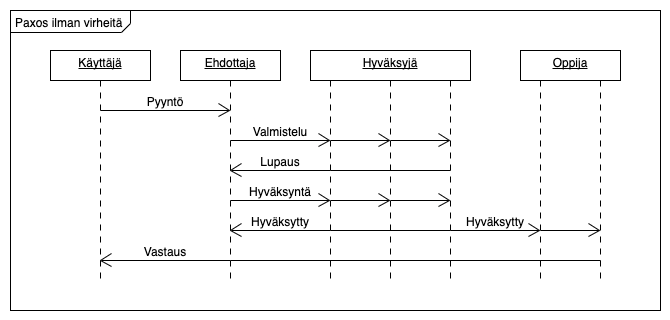
\includegraphics[height=6cm,keepaspectratio]{PaxosDiag}
%DIFDELCMD <   %%%
%DIFDELCMD < \caption[Yksinkertaistettu Paxos algoritmi]{%
{%DIFAUXCMD
\DIFdelFL{Yksinkertaistettu Paxos algoritmi}}
  %DIFAUXCMD
%DIFDELCMD < \label{fig:Paxos}
%DIFDELCMD < \end{figure}
%DIFDELCMD < 

%DIFDELCMD < %%%
\DIFdelend Raft algoritmi yrittää tehdä Paxos algoritmista lähestyttävämmän ja helpommin ymmärrettävän. Raft saavuttaa saman suoritustehon Paxos, mutta pienemmällä törmäystoleranssilla \parencite{panda2019study}. 
Koska Raft on arkitehtuuriltaa samanlainen kuin Paxos, Raft sisältää saman keskitetyn hallitsevan johtajan ongelman.

\section{Käytettävyyden tarkastelu}
Parhaimmat vaihtoehdot hajautetulle internetille ovat PoP, Paxos ja PoAh konsensus algoritmit \parencite{zarrin2021blockchain}. 
PoP tarvitsee vähän muistia ja laskentatehoa.
PoP algoritmilla on yhteys semanttiseen teknologiaan tarjoamalla identiteetteja datarakenteiden ominaisuuksille.
Paxos on toinen hyvä vaihtoehto sovellettavuuden takia. Paxos algoritmia adaptoitu moniin erilaisiin järjestelmiin, mikä tekee Paxos algoritmista hyvämaineisen uudelleenkohdennukseen.
Vaikka Paxosen protokollaa ja toteutettavuutta on vaikea ymmärtää. Jotta olisi hyvä vaihtoehto, tulisi algoritmia muokata lohkoketjuja varten.
PoAH algoritmi täyttää hajautetun internetin kriteerit olemassa vakaa, skaalautuva ja tarpeeksi tietoturvallinen. PoAH algoritmin luottamusjärjestelmä on tehokas työväline luotettavien nodejen luomiseen samalla pitäen nodet samanarvoisina järjestelmässä
\DIFdelbegin \DIFdel{.
}\DIFdelend 

\DIFaddbegin \begin{figure}[h]\centering
  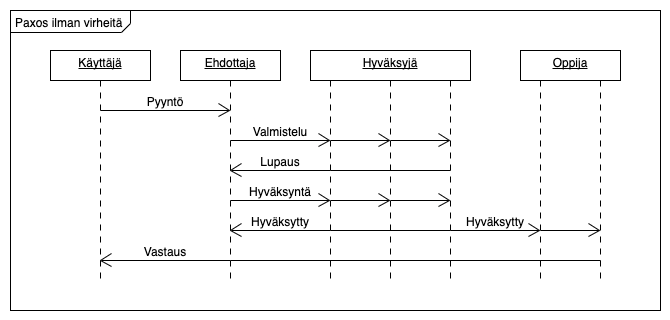
\includegraphics[height=6cm,keepaspectratio]{PaxosDiag}
  \caption[Yksinkertaistettu Paxos algoritmi]{\DIFaddFL{Yksinkertaistettu Paxos algoritmi}}
  \label{fig:Paxos}
\end{figure}

\DIFaddend \chapter{Lohkoketjujen haasteet}\label{Haasteet}

\section{Hallinto ja sääntely}
Jos lohkoketjut otetaan globaalisti käyttöön, keskitetyt regulaatiojärjestöt, kuten hallinnoillisetjärjestöt ja kansainväliset korporaatiot eivät pysty hallitsemaan lohkoketjuihin perustuvia aktiviteetteja. \parencite{wright2015decentralized}
Koska lohkoketjuilla ei ole tiettyä lokaatiota ja jokainen node voi olla eri geologisten toimivaltojen alaisuudessa ja täten heitä voi koskea eri lait. 
Kun ei ole keskitettyä hallintoa jokaiselle hajautetulle tilikirjalle, jolloin alueelliset regulaatiot muodostovat ongelman. \parencite{cermeno2016blockchain}
Olisi hyvä perustaa kansainväliset standardit lohkoketjujen terminologille, yhteentoimivuudelle, käyttäjän yksityisyydelle, tietoturvalle, käyttäjäidentiteetille, hallinnolle ja riskejä sisältäviin ongelmiin, milloin ihmiset saisivat enemmän luottoa lohkoketjuihin perustuviin yrityksiin \parencite{ali2019blockchain}.

\section{GDPR}

The European General Data Protection Regulation, lyhyemmin GDPR otettiin käyttöön 2016 \parencite{GDPR}.
GDPR antaa käyttäjille tiettyjä oikeuksia, kun he käyttävät verkkopalvelu, joissa palvelu käyttää käyttäjän dataa. Oikeudet sisältävät seuraavat kohdat.

Käyttäjälle tulee kertoa miten heidän henkilökohtaista dataansa tullaan käsittelemmään.
Käyttäjällä tulee olla pääsy heistä kerättyyn dataan.
Jos käyttäjä löytää väärää tietoa palvelun keräämässä datassa, käyttäjä pystyy liputtamaan kiistanalaisen datan.
Käyttäjän on saada yrityksen poistamaan kaikki käyttäjään liittyvät tiedot.
Jos käyttäjä arvioi dataansa, käyttäjän tulee pystyä rajoittomaan pääsyä tietoihinsa  arvioinin ajaksi.
Käyttäjän tulee pystyä vastustamaan datansa käyttöä, jos käyttäjä on erimieltä joidenkin automatisoitujen valintojen kanssa joihin käyttäjä sisältyy.

GDRP määrittelee kaksi määritelmää, rekisterinpitäjä ja tietojen käsittelijä, mitkä vaativat erityista huolellisuutta kun työskennellään lohkoketjuprojektien parissa. Molemman määritelmät liittyvät käyttäjän tietojen käsittelyyn käyttäjän luvalla.
Rekisterinpitäjä on se joka asettaa tietojenkäsittelylle tarkoitusperät ja keinot. Tietojenkäsittelijät taas ovat niitä henkilöitä tai yrityksiä, jotka käsittelevät käyttäjätietoja rekisterinpitäjän puolesta. Rekisterinpitäjällä ja tietojekäsittelijällä välillä tulee olla selkeä sopimus, jossa selitetään molempien osapuolien roolit ja funktiot.
Hajautetussa lohkoketjuympäristössä on tärkeä kysymys liittyy siihen kuka saa olla rekisterinpitäjä ja kuka tietojenkäsittelijä.

GDPR asettama oikeus tulla unohdetuksi -säädös aiheuttaa haassteita, koska käyttäjän tiedot on tallennettu lohkoketjussa useaan eri nodeen, ja täten yrityksen on vaikea ellei lähes mahdotonta poistaa data. On kuitenkin ehdotettu yhdeksi ratkaisuksi on kryptata jokainen lohkoketjun tallennus avainpareilla ja sisällyttää kryptattutieto lohkoketjuun. Tällöin poistamalla vastaava avain, kellään ei ole pääsyä kyseiseen lohkonsisältöön. Kuintenkaan kaikkialla ei ole juridisesti hyväksytty tämän kaltaista "poistamista". \parencite{ali2019blockchain}

\section{Skaalautuvuus}
Skaalautuvuus on yksi isoimmista lohkoketjuteknologioiden ongelmista. Skaalautuvuus ongelma voidaan jakaan kahteen osaan, transaktioiden tehokkuuteen ja \DIFdelbegin \DIFdel{tilantarpeeseen}\DIFdelend \DIFaddbegin \DIFadd{muistin tarpeeseen}\DIFaddend .

Lohkoketjusovellukset ovat yleensä itsehallittuja ja hyväksyvät transaktiolohkoja satunnaisin väliajoin.
Suoritusteho tälläisissä lohkoissa perustuu useinmiten lohkojen aikaväleihin ja lohkon maksimikokoon.
Lohkojen kasvattaminen tarkoittaa korkeampaa transaktioiden suoritustehoa, mutta samalla se tarkoittaa, että suuremmat lohkot tarvitsevat enemmän aikaa saavuttaakseen verkon nodet, aiheuttaen suuremman latenssin lohkojen sisällyttämiseen ja konsensus-algoritmeihin.
Toisaalta latenssi pienentyisi pienimmällä lohkon lisäysintervalilla, mutta tämä aiheuttaisi  enemmän erehdyksiä konsensus järjestelmässä.

Lohkonkoon skaalautuvuuden lisäksi nodejen muistin määrä skaalautuvuus on ongelma. Transaktioiden nopeus on suorassa yhteydessä osallistuvien nodejen muistin määrään.
Mitä enemmän nodeja liittyy lohkoketjuverkkoon sitä enemmän todennäköisesti transaktioita tullaan tekemään ja nodet tulee tarvitsemaan täten enemmän muistia.
Tulevaisuudessa on mahdollista että lohkoketjuteknologioita käyttävät useat miljoonat käyttäjät ja transaktioiden määrä kasvaa huomattavasti.
Koska hajautettu muisti on lohkoketjuille tyypillinen ominaisuus, muistinodeille kertyy valtavasti painetta, joka voi johtaa kasvavaan synkronointiviiveeseen ja energian kulutukseen.

%Skaalautuvuus ongelmaa voidaan ratkaista jonkin verran jakamalla transaktioiden suoritusprosessia moneen eri osaan.
%Varmistaaksemme skaalautuvuuden, transaktioiden suorittaminen voitaisiin suorittaa lohkoketjun ulkopuolella, missä kuitenkin transaktion hyväksyminen tapahtuisi lohkoketjuverkossa.
%Tämä ratkaisu vähentäisi transaktioiden varmennusaikaa. Esimerkiksi Bitcoinin päällä toimiva salamaverkko pystyy suorittamaan 45000 transaktiota sekuntissa, suorittamalla transaktioita lohkoketjun ulkopuolella.

\section{Suorituskyky}
Lohkoketjuteknologiat sisältävät useita suorituskykyyn liittyviä ongelmia, mitkä tekevät lohkoketjusta hitaan ja skaalautumattoman isoja transaktioita varten.
Ensimmäinen ongelma on älysopimukset. Älysopimuksissa on ongelmana niiden tehoton tiedonsiirto nodejen välillä. Myös se ettei pystytä ottaan käyttöön mielivaltaisia ohjelmia, jotka olisivat rajoitettu tiettyjen lohkojen muuttumattomuudella \parencite{yang2019survey}.
Toinen ongelma on lohkoketjun haarauttaminen, jossa eriävä haara muodostetaan lohkoketjusta, missä kyseisen lohkoketjun lohkoja louhutaan samanaikaisesti monien nodejen toimesta \parencite{da2019analysis}. 
Haarautus aiheittaa verkkoon viivettä yli 1000 s \parencite{mivsic2019forks}.
Haarautus sisältää myös tietoturvariskin, missä uuteen ketjuun, joka on luotu haarasta, pystytään upottamaan takaportteja \parencite{wang2019corking}.
Kolmas ongelma aiheuttaa pullonkaulan suorituskyvyssä. Pullonkaula aiheutuu lohkokoon seitsemään rajatusta transaktion pitkästä varmennusajasta \parencite{yang2019survey}.


\section{Tietoturvallisuus}
Vaikka lohkoketjujen transaktiot ovat suunnitellusti tietoturvallisia, yksityisyys pysyy huolen aiheena.
Lohkoketjuteknologioita ollaan pidetty yksityisyyden säilöjänä ja saanut hyvät arvostelut kyseisessa kontekstissä \parencite{de2016interplay}.
Kuitenkin kolmannen osapuolen web jäljittäjät ovat havainnnoineet kryptovaluuttojen deanonymisoituja käyttäjiä. Jäljittäjät hakevat käyttäjän identiteetin ja ostohistorian verkkokaupoista. Yleensä jäljittäjillä on tarpeeksi tietoa, jotta pystyvät tunnistamaam tietyn transaktion käyttäjän identiteetin mukana. 
Yleisesti uskotaan että lohkoketju on turvallinen, koska transaktiot suoritetaan generoiduilla osoitteilla kuin oikeilla identiteeteillä.
Ollaan näytetty etteivät lohkoketjutransaktiot takaa yksityisyyttä, koska transaktioiden saldot ja arvot on kaikkien saatavilla julkisista avaimista huolimatta \parencite{kosba2016hawk}.

On myös uhkia, jotka perustuu lohkoketjujen toimintaan. Yksi tietoturvallisuutta uhkaava hyökkäys on 51\% hyökkäys. 51\% hyökkäyksessa loujija omistaa yli puolet lohkoketjuverkon nodejen laskentatehosta. Tällöin kyseinen louhija pystyy dominoimaan järjestelmää mitä tulee transaktioiden luontiin, hyväksymiseen ja varmentamiseen tulee ja täten lisää vilpillisten transaktioden määrää.

Itsekkään louhijan hyökkäys on toinen yleinen hyökkäys. Hyökkäyksessä louhija generoi kaksi lohkoa, mutta ei julkaise niitä muille lohkoketjuverkon nodeille. Itsekäs louhija julkaisee lohkot vasta kuin lohkoketjuverkon muut nodet ovat liittäneet uuden lohkon ketjuun. Tällöin itsekkäällä louhijalla on lohkoketjun pisin ketju, jolloin aikaisemmin julkaistu lohko poistetaan ketjusta. Itsekäs louhija saa tällöin huomattavasti enemmän louhintapalkkiota \parencite{zheng2017overview}. 

% \section{Anonyymeys}



 \chapter{Yhteenveto}

 Lohkoketjuissa on vielä paljon ongelmia, mutta suurimpaan osaan on joitakin ratkaisuja.
 Konsensus-algoritmit ovat merkittävässä osassa lohkoketjuteknologioiden tehokkuudessa\DIFdelbegin \DIFdel{ja }\DIFdelend \DIFaddbegin \DIFadd{.
 }\DIFaddend PoP, Paxos, PoAH \DIFdelbegin \DIFdel{vaikuttaa }\DIFdelend \DIFaddbegin \DIFadd{vaikuttavat }\DIFaddend olevan merkittävässä osassa lohkoketjujen kehitystä.

 
 


\printbibliography

\appendix


\end{document}
